\documentclass[a4paper,12pt]{jsbook}
\setlength{\textwidth}{\fullwidth}
\setlength{\evensidemargin}{\oddsidemargin}
\usepackage{thesis}
\usepackage{makeidx}
\usepackage{amsmath}
\usepackage{txfonts, float}
\usepackage{here}
\usepackage[dvipdfmx]{graphicx}
\usepackage[noto-otc, unicode]{pxchfon}

\begin{document}

% 表紙
\thesis{
\scalebox{}{\bf 20XX年度} \\
\scalebox{}{\bf 修\quad 士\quad 論\quad 文}
}
\date{20xx年xx月xx日}
\title{
    \vspace{1.2zh}
    \scalebox{0.9}{研究タイトル}
}
\teacher{\quad 尾上\quad 洋介\quad 准教授}
\organization{
    日本大学大学院総合基礎科学研究科\\
    地球情報数理科学専攻\\
    情報科学部門}
\author{
\scalebox{1}{名字 \quad 名前} \\
}

\maketitle

% 前書き
\chapter*{概要}
\thispagestyle{empty}

\frontmatter
\tableofcontents
\listoffigures
\listoftables

% 本文
\mainmatter
\chapter{How To Use \LaTeX}

\section{Figure}
    \subsection{基本的な画像挿入方法}
    写真はimg下に配置します.\\
    \begin{figure}[htbp]
        \centering   
        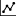
\includegraphics[width=0.5\textwidth]{img/sample/sample_png.png}
        \label{fig:sample_png}
        \caption[sample image (png)]{sample image: when its extension is png.}
    \end{figure}
    labelで指定することで, \figref{fig:sample_png}はxxxのように参照することができる.\\
    captionでは [] が目次に示される内容で, \{\} が本文に示される内容である. 同じでいい場合は \{\} のみで良い.\\
    上記のように, pngやjpegのようなラスタ画像を用いると, 拡大したときに荒くなってしまう.\\
    下記のようにpdfのようなベクタ画像を用いると拡大しても荒くならない.
    ただし, 保存時にベクタ形式にする必要がある.
    \begin{figure}[htbp]
        \centering   
        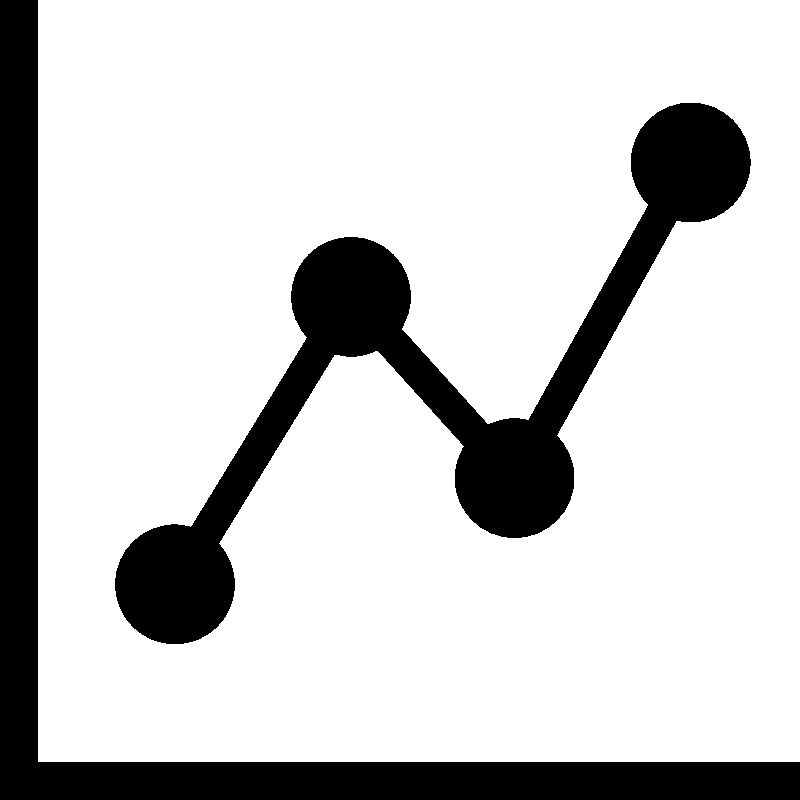
\includegraphics[width=0.5\textwidth]{img/sample/sample_pdf.pdf}
        \label{Fig:sample_pdf}
        \caption[sample image (pdf)]{sample image: when its extension is pdf.}
    \end{figure}
    出力の位置は[htbp]で指定するが, レイアウトによっては自動的に次のページに移動するなど, 指定した通りに配置できないときがある.\\
    この場合は[H]のように大文字で指定すると,
    \begin{figure}[H]
        \centering   
        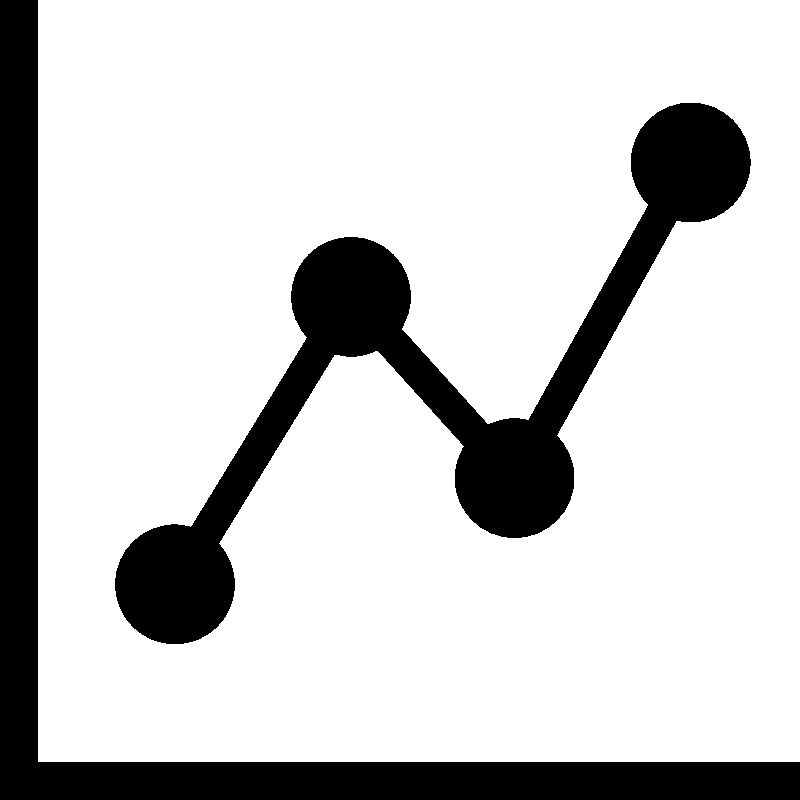
\includegraphics[width=0.5\textwidth]{img/sample/sample_pdf.pdf}
        \label{Fig:sample_pdf_here}
        \caption[sample image (pdf, here)]{sample image: when its extension is pdf and is enforced to be here.}
    \end{figure}
    このように強制的に配置が可能になる.

    \subsection{複数画像の挿入}
    複数画像の挿入方法はいくつかあるようだが, とりあえず下記で挿入することが可能.
    \begin{figure}[H]
		\centering
		\begin{tabular}{c}
		% ----- image 1 =====
			\begin{minipage}{0.25\hsize}
				\centering
				
\includegraphics[width=\textwidth]{img/sample/sample1.pdf}
				\text{(a)}
			\end{minipage}
		% ----- image 2 =====
			\begin{minipage}{0.25\hsize}
				\centering
				
\includegraphics[width=\textwidth]{img/sample/sample2.pdf}
				\text{(b)}
			\end{minipage}
		% ----- image 3 =====
			\begin{minipage}{0.25\hsize}
				\centering
				
\includegraphics[width=\textwidth]{img/sample/sample3.pdf}
				\text{(c)}
			\end{minipage}
		% ----- image 4 =====
			\begin{minipage}{0.25\hsize}
				\centering
				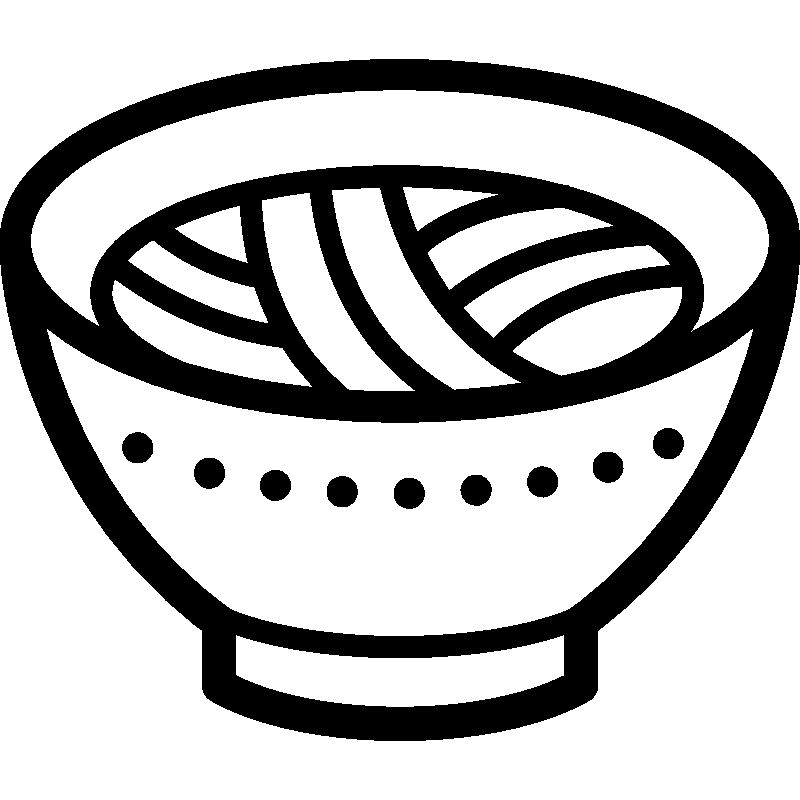
\includegraphics[width=\textwidth]{img/sample/sample4.pdf}
				\text{(d)}
			\end{minipage}
		\end{tabular}
		\caption[Four sample images]
		{
			Four sample images.
			(a) sushi (b) milk (c) peach (d) ramen
		}
		\label{fig:sample_four_images}
	\end{figure}

    縦2横2にすることも可能.
    \begin{figure}[H]
		\centering
		\begin{tabular}{c}
		% ----- image 1 =====
			\begin{minipage}{0.25\hsize}
				\centering
				
\includegraphics[width=\textwidth]{img/sample/sample1.pdf}
				\text{(a)}
			\end{minipage}
			\hspace{1cm}
		% ----- image 2 =====
			\begin{minipage}{0.25\hsize}
				\centering
				
\includegraphics[width=\textwidth]{img/sample/sample2.pdf}
				\text{(b)}
			\end{minipage}
			\vspace{1cm}\\
		% ----- image 3 =====
			\begin{minipage}{0.25\hsize}
				\centering
				
\includegraphics[width=\textwidth]{img/sample/sample3.pdf}
				\text{(c)}
			\end{minipage}
			\hspace{1cm}
		% ----- image 4 =====
			\begin{minipage}{0.25\hsize}
				\centering
				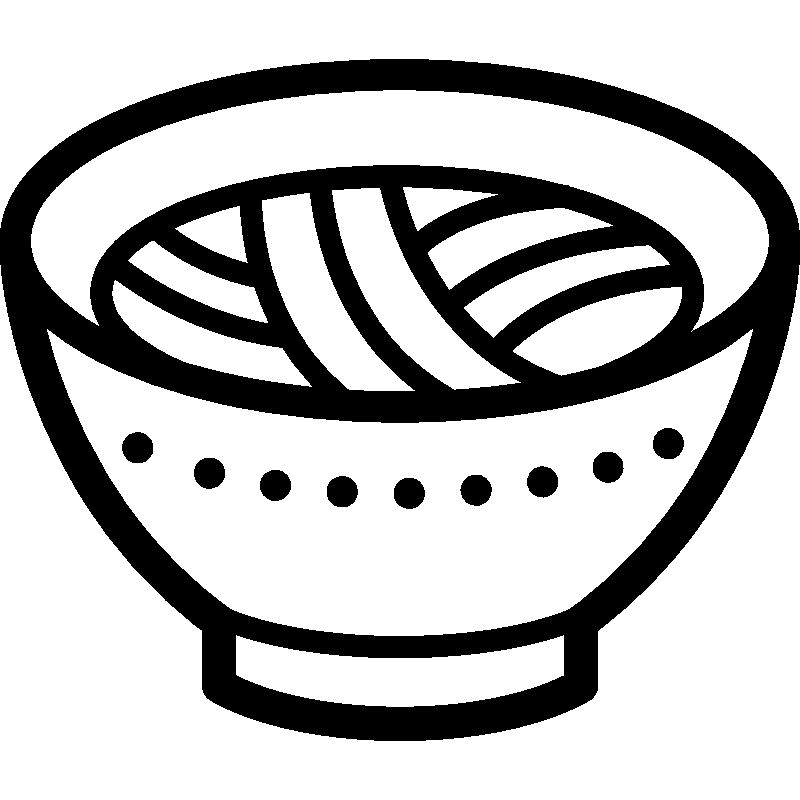
\includegraphics[width=\textwidth]{img/sample/sample4.pdf}
				\text{(d)}
			\end{minipage}
		\end{tabular}
		\caption[Four sample images]
		{
			Four sample images 2.
			(a) sushi (b) milk (c) peach (d) ramen
		}
		\label{fig:sample_four_images2}
	\end{figure}
    
\section{Table}
Tableは\tbref{tb:sample_table}のようにして挿入する.
\begin{table}[H]
	\centering
	\caption{Sample Table: accuracy for train/evaluation data.}
	\begin{tabular}{ll}\hline
		 訓練データの正答率&: $98\%$ \\
		 テストデータの正答率&: $88\%$ \\
	\label{tb:sample_table}
	\end{tabular}
\end{table}

\section{Bib}
参考文献は, \cite{author:06}とすれば良い.
複数の参考文献を扱う場合は, \cite{author:06, conference:06}のようにする.\\
使用してない参考文献は自動的に記載されないようになっているので, とりあえずbib/liter.bibに入れておいて構わない.\\
通し番号は本文で言及された順になるがこれも自動的に処理されるので気にしなくて良い.

\section{Equation}
数式の入力はたくさんある.
文章中であれば, $x = 2$ のように挿入できる.\\
数式環境を用意する場合は, \equref{eq:sample1}, \equref{eq:sample2}, \equref{eq:sample3}のようにできる.

\begin{align}
    x &= 2 \label{eq:sample1}\\
    y &= x^2 + 1 \label{eq:sample2}\\
      &= 5 \label{eq:sample3}
\end{align} % 使い方を示す例
\chapter{序論}

\section{研究背景}

\section{本研究の目的と方法}

\section{本論文の構成}
本論文は本章を含め, 7つの章と2つの付録からなる.
\begin{itemize}
	\item 第1章では本論文の位置づけについて記した.
	\item 第2章では背景について記した.
	\item 第3章では提案手法について記した.
	\item 第4章では実験について記した.
	\item 第7章では提案手法に関して結論を考察し, 今後の展望に関して述べた.
	\item 付録Aではその他の本研究に関する予備実験や補足事項について述べた.
	\item 付録Bではその他の実験を載せた.
\end{itemize}
\chapter{背景}
\chapter{提案手法}
\chapter{実験結果}
\chapter{結論と展望}

\section{結論}
本研究の貢献は次の2つである.
\begin{itemize}
	\item your contribution 1
	\item your contribution 2
\end{itemize}

\section{課題と展望}
\chapter*{謝辞}
\addcontentsline{toc}{chapter}{謝辞}

本研究は, professor 教授のご指導のもとで行われました.
\bibliographystyle{bib/IEEEtransBST/IEEEtran}
\bibliography{bib/style,bib/liter}

\renewcommand{\prechaptername}{付録}
\renewcommand{\postchaptername}{}
\renewcommand{\thechapter}{\Alph{chapter}}
\setcounter{chapter}{0}

\chapter{実験の補足}
\renewcommand{\prechaptername}{付録}
\renewcommand{\postchaptername}{}
\renewcommand{\thechapter}{\Alph{chapter}}

\chapter{その他の実験}

% 後書き
\backmatter
\appendix

\printindex
\end{document}